% !TEX root = /tex/main.tex
\documentclass[11pt]{umtlreport}
\usepackage[utf8]{inputenc}
\usepackage[T1]{fontenc}
\usepackage[scaled=0.85]{helvet}
\usepackage[colorlinks=true,linkcolor=black,citecolor=black,urlcolor=black]{hyperref}
\usepackage{microtype}
\usepackage{fancyhdr}
\usepackage{graphicx}
\usepackage{palatino}
\usepackage{listings}
\usepackage{appendix}
\usepackage{remreset}
\usepackage{qtree}
\usepackage{wrapfig}
\usepackage{array}
\usepackage{multirow}
\usepackage{amsmath}
\usepackage{amssymb}
\usepackage{color}
\usepackage{subcaption}
\usepackage{amsfonts}   % for math fonts
\usepackage{calc}
\usepackage[natbibapa]{apacite}
\usepackage{floatrow}


\newlength\myheight
\newlength\mydepth
\settototalheight\myheight{Xygp}
\settodepth\mydepth{Xygp}
\setlength\fboxsep{0pt}
\newcommand*\inlinegraphics[1]{%
  \settototalheight\myheight{Xygp}%
  \settodepth\mydepth{Xygp}%
  \raisebox{-\mydepth}{\includegraphics[height=\myheight]{#1}}%
}
\makeatletter
\@removefromreset{footnote}{chapter}
\makeatother



\setlength{\headheight}{15.2pt}
\pagestyle{fancy}
\fancyhead[RO]{\thepage}
\fancyhead[LO]{}
\fancyfoot{}

\newcommand{\TODO}[1]{\hspace{-1.45cm}\textcolor{red}{ \textbf{TODO: #1}}}
\newcommand{\ITODO}[1]{\textcolor{red}{ \textbf{TODO: #1}}}
\newfloatcommand{capbtabbox}{table}[][\FBwidth]




\definecolor{orange}{rgb}{1,.49,.18}
\definecolor{darkgreen}{rgb}{0,.66,.0}
\definecolor{mypurple}{rgb}{.76,0,.83}
\newcommand{\var}[1]{{\color{orange} \textbf{#1}}}
\newcommand{\autovar}[1]{{\color{darkgreen} \textbf{#1}}}
\newcommand{\conj}[1]{{\color{mypurple} \textbf{#1}}}



\fancypagestyle{plain}{%
   \fancyhf{}%
   \fancyhead[C]{} %Kapitelname ausblenden

   \renewcommand{\headrulewidth}{0.0pt} %obere Linie ausblenden
   \fancyfoot[C]{\thepage}
}

\setcounter{secnumdepth}{2} 

\newcolumntype{C}[1]{wc{#1}} % fixed width & centered


\begin{document}

\lstset{language=Python, basicstyle=\footnotesize}

\renewcommand{\thepage}{\roman{page}}
\newcommand{\monthword}[1]{\ifcase#1\or January\or February\or March\or April\or
                                        May\or June\or July\or August\or
                                        September\or October\or November\or December\fi} 

\begin{titlepage}
\unitlength1mm

\begin{picture}(0,215)(0,0) %(0,0) is bottom left
 
%%%%%%%%%%%%%%%%%%HEAD START
\put(0,215){\rule{15cm}{0.1cm}}

\put(20,184){  
\parbox[b]{10cm}{
  \raggedleft{
  \fontsize{14}{18}\selectfont
   SAARLAND UNIVERSITY\\
	   ~\\
	 \fontfamily{ptm}\fontsize{12}{14}\selectfont Faculty of Mathematics and Computer Science\\
   Department of Computer Science\\
   BACHELOR THESIS\\
   Degree Program: Computer Science (English)
	}
}}

\put(125,184){
\includegraphics[height=28mm]{images/c0/uds_owl}}
\put(0,183){\rule{12.2cm}{0.025cm}} 


%%%%%%%%%%%%%%%%%%HEAD END



%%%%%%%%%%%%%%%%%%BODY START

\def\horizontalDistance{7}


\put(\horizontalDistance,95){\parbox[b]{128mm}{
 \sffamily\Huge
 \begin{center}
  Understanding Pragmatic Reasoning Through Eye
  Movement Patterns in Reference Games
 \end{center}
}}



\put(\horizontalDistance, 10){\parbox[b]{128mm}{
\begin{flushleft}

\begin{center}
\scriptsize
submitted by\\
\normalsize
Tymur Mykhalievskyi\\
Saarbrücken \\
\monthword{\month} \the\year
\end{center}
\end{flushleft}
}}

%%%%%%%%%%%%%%%%%%BODY END


%%%%%%%%%%%%%%%%%%BOTTOM START
\put(-35,0){\rule{3.5cm}{0.25cm}}
\put(0,0){\rule{15cm}{0.025cm}}
%%%%%%%%%%%%%%%%%%BOTTOM END

\end{picture}


\end{titlepage}


\pagestyle{empty}

\vspace*{0.5cm}
\textbf{Advisors:}\\
Prof. Dr. Vera Demberg\\
Computer Science and Computational Linguistics\\
Saarland University\\
Saarbrücken, Germany\\\\

Dr. John Duff\\
Computer Science and Computational Linguistics\\
Saarland University\\
Saarbrücken, Germany\\\\


\vspace*{2.5cm}
\textbf{\color{red}  Reviewer 1: ADD THE NAME}\\
\textbf{\color{red}  Reviewer 2: ADD THE NAME}\\


\vspace{4.5cm}

\textbf{\color{red}  Disclaimer: We provide this templates for your convenience. As we do not update it regularly, it is your responsibility to ensure that it complies with your examination office's rules. This is especially valid for the declarations that you need to formulate. We have not integrated them in this template on purpose. Please add this on your own, while checking the rest of the template with the current rules.}


\vspace{3cm}
Saarland University\\
Faculty MI – Mathematics and Computer Science\\
Department of Computer Science\\
Campus - Building E1.1\\
66123 Saarbrücken\\
Germany\\



\clearpage
\section*{Declarations}
I hereby confirm that the thesis presented here is my own work, with all assistance acknowledged. I assure that the electronic version is identical in content to the printed version of the thesis.

% skip some space for the signature
\vspace{2cm}


Tymur Mykhalievskyi

Saarbrücken, \today
\clearpage
\section*{Acknowledgements}

\clearpage
\section*{Abstract}

\clearpage

\begingroup
  \pagestyle{plain}

\setcounter{tocdepth}{2}
  \addtocontents{toc}{\protect\thispagestyle{plain}}
  \addtocontents{toc}{\protect\vspace{-.45cm}}
  \tableofcontents
  \clearpage
\endgroup 

\pagestyle{fancy}
\setcounter{page}{1}
\renewcommand{\thepage}{\arabic{page}}

\section*{Introduction} \label{sec:intro}
If one says ``I am going to Munich this week. My mother lives there.'', you will interpret this as meaning they are visiting their mother, even though it is not explicitly stated. This is called an implicature, without explicitly stating something one can still deliver the information. Human communication is full of such implicit constructions. One reason for this may be to save cognitive effort. What rules do people unconsciously follow during communication to make it more efficient?

In 1975 a British philosopher Paul Grice finalized four types of maxims \citep{Grice_1975}. Maxim of Quantity: Provide as much information as required, do not provide more information than required. Maxim of Quality: Be truthful, only say that for which you have adequate evidence. Maxim of Relation: be relevant. Maxim of Manner: avoid ambiguity. Going back to the example with traveling, we can assume a speaker is obeying the maxims. Therefore, the information is relevant and the right amount is provided, so the second sentence about where the mother lives is not just a disconnected fact. Hence, we build an implicature that one is visiting their mother.

One way to study this is through reference games. In these games, participants engage in a collaborative task, often involving the identification or description of objects, where effective communication and reasoning play key roles. Over the years, these reference games have become a popular experimental paradigm to explore how individuals reason about others' intentions and strategies in communication \citep{Frank_2012,Franke_2016}. A simple example is presented in \autoref{fig:intro_complex}. Imagine someone is talking to you and uses the word ``blue'' to refer to one of these objects. Which object are they talking about? If you answered blue square, congrats, it is considered the correct solution. Do not worry, if you are confused. If we consider the possibilities of the speaker, the two completely unambiguous messages available to them are ``green'' and ``circle''. Hence, if they would have referred to one of the other objects, there are clear messages to do that. Thus, we are left with messages ``blue'' and ``square''. Although the message ``blue'' corresponds to two objects, the blue circle can be referred to unambiguously by using message ``circle''. Similar logic can be applied to the message ``square''. So both of them can be inferred to point to the blue square. All this reasoning is built upon the Gricean maxims, as we expect from the speaker to be as concise, unambiguous, relevant and truthful as they can be. 

On the other hand, one could notice that the reference games are not as intuitive as the traveling example. It is still a limitation that we will have to keep for now. And this study could also shed light on this problem by understanding what exactly people are doing to solve this kind of problems.

In order to deepen the understanding, a formal model was developed, it is called Rational Speech Act model. It tries to mimic a recursive sequence of reasoning between speaker and listener \citep{Franke_2016}. Despite significant progress in understanding the cognitive processes underlying these tasks, much remains unknown about the specific strategies individuals employ when solving particular problems within these games.

This study seeks to expand on prior research by incorporating a novel dimension: tracking participants' eye gaze during reference games. Eye gaze offers valuable insight into how people process information, make decisions, and employ strategies. By capturing where and when participants direct their attention, we can gain a deeper understanding of the cognitive mechanisms at play, including how individuals prioritize certain visual cues and how these cues influence their reasoning strategies. This approach has shown to be a very insightful tool \citep{Vigneau_2006}.

In particular, this study aims to answer the question: How do gaze patterns correlate with the accuracy and strategies used to solve specific communicative challenges in reference games? By integrating eye-tracking data with the analysis of reasoning in these games, this paper contributes to a richer understanding of the decision-making processes involved in collaborative communication and problem-solving.

\begin{figure}
    \centering
    
\includegraphics[width=0.6\linewidth]{images/intro_complex.png}
    \caption{An example of reference game. Same example is shown in \cite{Frank_2012}. A speaker utters ``blue'', which object are they referring to?}
    \label{fig:intro_complex}
\end{figure}
\chapter{Related Work}
\section{Reference Games}
Although, the idea of communication as a signaling game goes back to \cite{Lewis_1969}, we will be focusing on a type of a signaling game called a reference game as presented in \cite{Frank_2012}. The game tries to mimic the challenges of communication that people face on daily basis, as we discussed in the \autoref{sec:intro}. At first, an instance of a reference game looked as in \autoref{fig:intro_complex}, that is, no information about the available messages is given to the speaker and listener. The later instances, on the other hand, include this information. The examples are shown in \autoref{fig:simple_complex}. The goal for newer version is the same, that is, to identify which object a speaker is referring to. This change allows for more controlled experiments by increasing the variability in setups. In addition, it should improve clarity, for instance, participants should not wonder, why wouldn't the speaker just utter the location of the object instead of specifying the properties.

\begin{figure}
\centering
\begin{subfigure}{.5\textwidth}
  \centering
  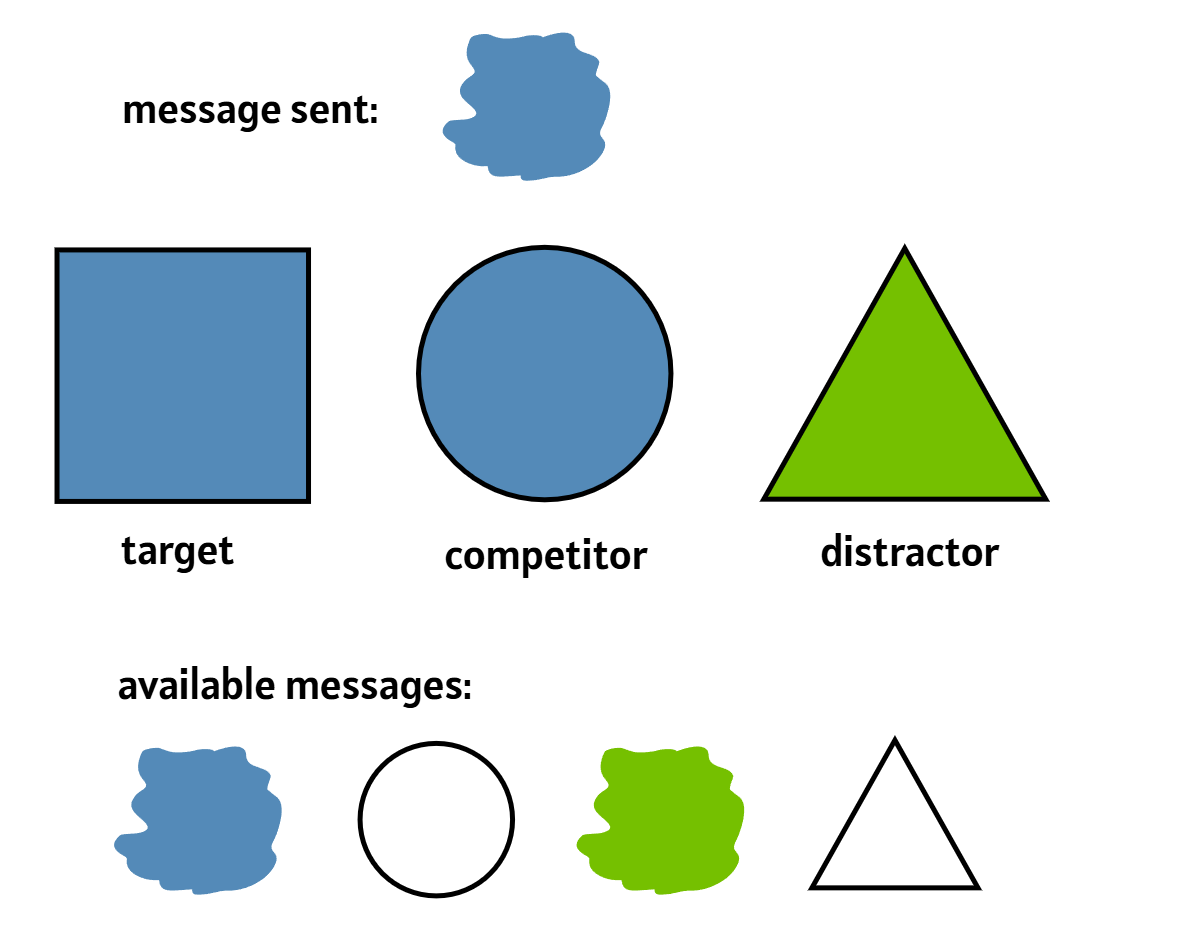
\includegraphics[width=1\linewidth]{images/simple.png}
  \caption{simple}
  \label{fig:simple}
\end{subfigure}%
\begin{subfigure}{.5\textwidth}
  \centering
  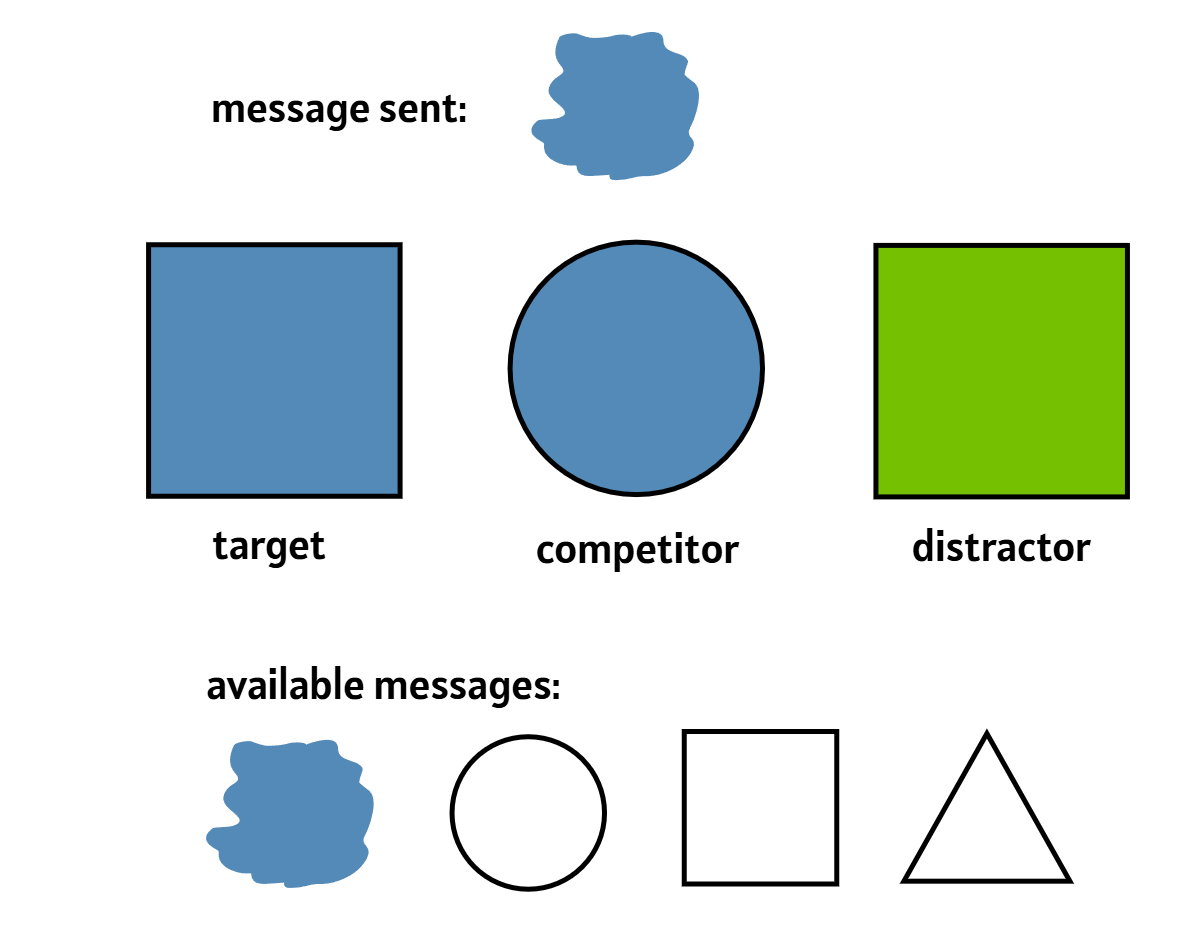
\includegraphics[width=1\linewidth]{images/complex.png}
  \caption{complex}
  \label{fig:complex}
\end{subfigure}
\caption{Two instances of reference games with different difficulties. }
\label{fig:simple_complex}
\end{figure}

Let's take a closer look at \autoref{fig:simple}. An uttered message is presented on the top. We will denote the object being referred to as a target, a competitor is an object that shares the message property with the target. While a distractor does not share the sent message property, but could share another property with the target depending on the difficulty of the trial. Note that, obviously, captions target, competitor and distractor are not available to the participants. The difference between the simple and complex trials in \autoref{fig:simple_complex} mainly in how the distractor is constructed. In particular, in the simple trial it does not share any properties with the target, while in the complex it does. The simple example \autoref{fig:simple} can be solved without considering the distractor. That is, one could count the matching messages from the available ones. In this case, it would be 1 for blue square, 2 for blue circle and 2 for green triangle. Hence, the target is blue square, as ``blue'' is the only message that could refer to it. This way of solving is not necessarily what people tend to do, but it is one way of interpreting the difference between simple and complex trials. Because if you apply the same strategy to the complex example in \autoref{fig:complex}, both target and competitor have two matching messages. On the other hand, if you try to solve these examples yourself, you will probably end up recursively reasoning of what the speaker could have said had they had another target. The simple and complex in this case still appear to their names, you will need a more robust recursion in order to solve the complex one comparing to the simple one.

\section{Rational Speech Act Model} \label{sec:rsa}
Studying this phenomena needs a formalized approach. One such model, called the Rational Speech Act (RSA) was developed. It mimics how a speaker and a listener reason about each other. A detailed explanation can be found in the manuscript by \cite{Frank_2016} as well as in the article \cite{Franke_2016}. We will go through the main ideas of how listener and speaker interact with each other. Firstly, take a look at the matrix $M_s$ from the \autoref{eq:1}. Each columns is a one-hot encoding of an objects, in other words this matrix encodes which objects match the literal meaning of each message, this matrix is constructed for the simple example in \autoref{fig:simple}. 
\begin{equation} \label{eq:1}
M_s = \!\!\!\!
\raisebox{2.3ex}{$
\begin{array}{c@{\;}c}
    & {
    \begin{array}{*{4}{C{20pt}}} 
        \inlinegraphics{images/shapes_and_colors/blue_square.png} & \inlinegraphics{images/shapes_and_colors/blue_circle.png} & \inlinegraphics{images/shapes_and_colors/green_triangle.png}  
      \end{array}} \\[5pt]
    \begin{array}{c} 
        \inlinegraphics{images/shapes_and_colors/blue.png} \\ 
        \inlinegraphics{images/shapes_and_colors/circle.png} \\ 
        \inlinegraphics{images/shapes_and_colors/green.png} \\
        \inlinegraphics{images/shapes_and_colors/triangle.png}
    \end{array} 
    & 
    \left[
    \begin{array}{*{3}{C{20pt}}}
        1 & 1 & 0  \\
        0 & 1 & 0  \\
        0 & 0 & 1  \\
        0 & 0 & 1  \\
    \end{array} \right]
\end{array}$
}
\end{equation}

Now let us define a listener matrix, each row shows conditional probabilities for the objects given a message. Accordingly a speaker matrix has columns that depict conditional probabilities of messages given an object. 

Subsequently we arrive at a literal listener \autoref{eq:2} and speaker \autoref{eq:3}. Simply put a literal speaker would output one of the matching messages with equal probability for the given target. For example, if green triangle is provided for the speaker, they would refer to it be uttering ``green'' or ``triangle'' with equal probability. While literal listener would interpret the ambiguous messages with equal probabilities.

\begin{equation} \label{eq:2}
L_0(M_s)=L(M_s) =\!\!\!\!
\raisebox{2.3ex}{$
\begin{array}{c@{\;}c}
    & {
    \begin{array}{*{3}{C{20pt}}} 
        \inlinegraphics{images/shapes_and_colors/blue_square.png} & \inlinegraphics{images/shapes_and_colors/blue_circle.png} & \inlinegraphics{images/shapes_and_colors/green_triangle.png}  
      \end{array}} \\[5pt]
    \begin{array}{c} 
        \inlinegraphics{images/shapes_and_colors/blue.png} \\ 
        \inlinegraphics{images/shapes_and_colors/circle.png} \\ 
        \inlinegraphics{images/shapes_and_colors/green.png} \\
        \inlinegraphics{images/shapes_and_colors/triangle.png}
    \end{array} 
    & 
    \left[
    \begin{array}{*{3}{C{20pt}}}
        0.5 & 0.5 & 0  \\
        0 & 1 & 0  \\
        0 & 0 & 1  \\
        0 & 0 & 1  \\
    \end{array} \right]
\end{array}$
}
\end{equation}

\begin{equation} \label{eq:3}
S_0(M_s)=S(M_s) = \!\!\!\!
\raisebox{2.3ex}{$
\begin{array}{c@{\;}c}
    & {
    \begin{array}{*{4}{C{20pt}}} 
        \inlinegraphics{images/shapes_and_colors/blue_square.png} & \inlinegraphics{images/shapes_and_colors/blue_circle.png} & \inlinegraphics{images/shapes_and_colors/green_triangle.png}  
      \end{array}} \\[5pt]
    \begin{array}{c} 
        \inlinegraphics{images/shapes_and_colors/blue.png} \\ 
        \inlinegraphics{images/shapes_and_colors/circle.png} \\ 
        \inlinegraphics{images/shapes_and_colors/green.png} \\
        \inlinegraphics{images/shapes_and_colors/triangle.png}
    \end{array} 
    & 
    \left[
    \begin{array}{*{3}{C{20pt}}}
        1 & 0.5 & 0  \\
        0 & 0.5 & 0  \\
        0 & 0 & 0.5  \\
        0 & 0 & 0.5  \\
    \end{array} \right]
\end{array}$
}
\end{equation}

One could see that such approach would not solve even a simple trial. However, if there is a completely unambiguous message, the literal listener would be able to correctly identify the target. The way we derived the two matrices is just a normalization within columns or rows, correspondingly for the listener and speaker.  We can keep applying this technique recursively, to find more complex listeners and speakers. That is, a speaker would normalize within columns the matrix previously normalized within rows. In this way we can derive an $L_1$ listener \autoref{eq:4}, also called a first-order cooperative listener. Note that \cite{Frank_2016} and \cite{Franke_2016} apply different strategies to construct $L_1$ and $L_2$ listeners, we will stick to the \cite{Franke_2016} variation.

\begin{equation} \label{eq:4}
L_1(M_s)=L(S(M_s)) = \!\!\!\!
\raisebox{2.3ex}{$
\begin{array}{c@{\;}c}
    & {
    \begin{array}{*{4}{C{20pt}}} 
        \inlinegraphics{images/shapes_and_colors/blue_square.png} & \inlinegraphics{images/shapes_and_colors/blue_circle.png} & \inlinegraphics{images/shapes_and_colors/green_triangle.png}  
      \end{array}} \\[5pt]
    \begin{array}{c} 
        \inlinegraphics{images/shapes_and_colors/blue.png} \\ 
        \inlinegraphics{images/shapes_and_colors/circle.png} \\ 
        \inlinegraphics{images/shapes_and_colors/green.png} \\
        \inlinegraphics{images/shapes_and_colors/triangle.png}
    \end{array} 
    & 
    \left[
    \begin{array}{*{3}{C{20pt}}}
        0.66 & 0.33 & 0  \\
        0 & 1 & 0  \\
        0 & 0 & 1  \\
        0 & 0 & 1  \\
    \end{array} \right]
\end{array}$
}
\end{equation}

$L_1$ listener gives the highest probability to the target with message blue. Repeating this procedure further to get to deeper recursion increases the probability of target being chosen. In addition, RSA model has a greed parameter $\alpha$ which amplifies the probabilities. $\alpha=\infty$ would result in simply choosing the object with the highest probability. Now let's take a look at the complex case and see how it differs from the simple one. The matrix $M_c$ is given in \autoref{eq:5}.

\begin{equation} \label{eq:5}
M_c = \!\!\!\!
\raisebox{2.3ex}{$
\begin{array}{c@{\;}c}
    & {
    \begin{array}{*{4}{C{20pt}}} 
        \inlinegraphics{images/shapes_and_colors/blue_square.png} & \inlinegraphics{images/shapes_and_colors/blue_circle.png} & \inlinegraphics{images/shapes_and_colors/green_square.png}  
      \end{array}} \\[5pt]
    \begin{array}{c} 
        \inlinegraphics{images/shapes_and_colors/blue.png} \\ 
        \inlinegraphics{images/shapes_and_colors/circle.png} \\ 
        \inlinegraphics{images/shapes_and_colors/square.png} \\
        \inlinegraphics{images/shapes_and_colors/triangle.png}
    \end{array} 
    & 
    \left[
    \begin{array}{*{3}{C{20pt}}}
        1 & 1 & 0  \\
        0 & 1 & 0  \\
        1 & 0 & 1  \\
        0 & 0 & 0  \\
    \end{array} \right]
\end{array}$
}
\end{equation}

Going through the same steps to derive the $L_1$ listener, we get \autoref{eq:6}. 

\begin{equation} \label{eq:6}
L_1(M_c) = L(S(M_c)) = \!\!\!\!
\raisebox{2.3ex}{$
\begin{array}{c@{\;}c}
    & {
    \begin{array}{*{3}{C{20pt}}} 
        \inlinegraphics{images/shapes_and_colors/blue_square.png} & \inlinegraphics{images/shapes_and_colors/blue_circle.png} & \inlinegraphics{images/shapes_and_colors/green_square.png}  
      \end{array}} \\[5pt]
    \begin{array}{c} 
        \inlinegraphics{images/shapes_and_colors/blue.png} \\ 
        \inlinegraphics{images/shapes_and_colors/circle.png} \\ 
        \inlinegraphics{images/shapes_and_colors/square.png} \\
        \inlinegraphics{images/shapes_and_colors/triangle.png}
    \end{array} 
    & 
    \left[
    \begin{array}{*{3}{C{20pt}}}
        0.5 & 0.5 & 0  \\
        0 & 1 & 0  \\
        0.33 & 0 & 0.66  \\
        0 & 0 & 0  \\
    \end{array} \right]
\end{array}$
}
\end{equation}

One important difference is that depth of recursion for the $L_1$ listener is not enough to assign the highest probability to the target. Here the ``blue'' row has the same probabilities for the distractor and the target. Note that in this case the greed parameter $\alpha$ would not be able to help. So instead we consider a deeper level of recursion and introduce an $L_2$ listener \autoref{eq:7}, also called second-order cooperative listener. 

\begin{equation} \label{eq:7}
L_2(M_c) = L(S(L(M_c))) = \!\!\!\!
\raisebox{2.3ex}{$
\begin{array}{c@{\;}c}
    & {
    \begin{array}{*{4}{C{20pt}}} 
        \inlinegraphics{images/shapes_and_colors/blue_square.png} & \inlinegraphics{images/shapes_and_colors/blue_circle.png} & \inlinegraphics{images/shapes_and_colors/green_square.png}  
      \end{array}} \\[5pt]
    \begin{array}{c} 
        \inlinegraphics{images/shapes_and_colors/blue.png} \\ 
        \inlinegraphics{images/shapes_and_colors/circle.png} \\ 
        \inlinegraphics{images/shapes_and_colors/square.png} \\
        \inlinegraphics{images/shapes_and_colors/triangle.png}
    \end{array} 
    & 
    \left[
    \begin{array}{*{3}{C{20pt}}}
        0.6 & 0.4 & 0  \\
        0 & 1 & 0  \\
        0.33 & 0 & 0.66  \\
        0 & 0 & 0  \\
    \end{array} \right]
\end{array}$
}
\end{equation}

\begin{figure}
\centering
\begin{subfigure}{.5\textwidth}
  \centering
  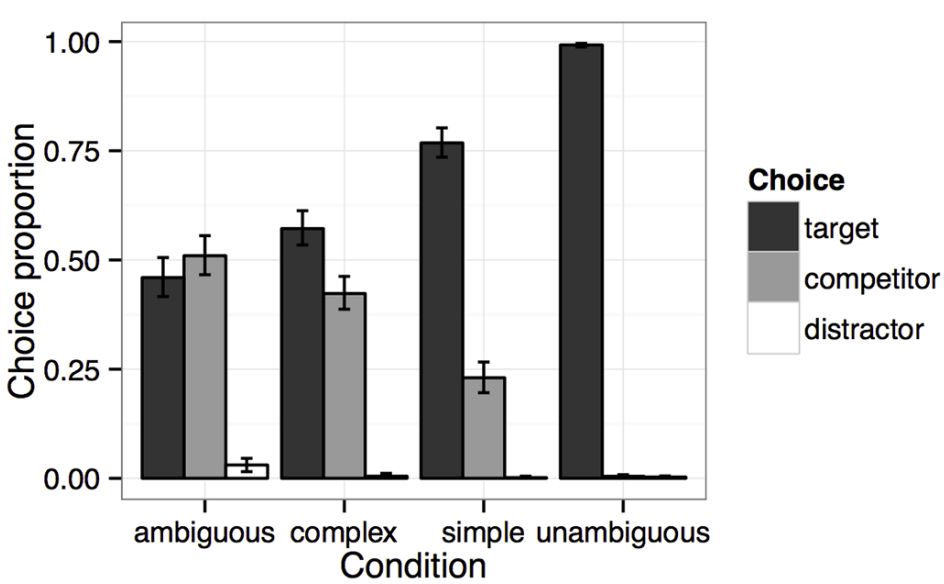
\includegraphics[width=1\linewidth]{images/trials_stats.png}
  \caption{Proportions of target, competitor and distractor choices in their experiment. }
  \label{fig:trial_stats}
\end{subfigure}%
\begin{subfigure}{.5\textwidth}
  \centering
  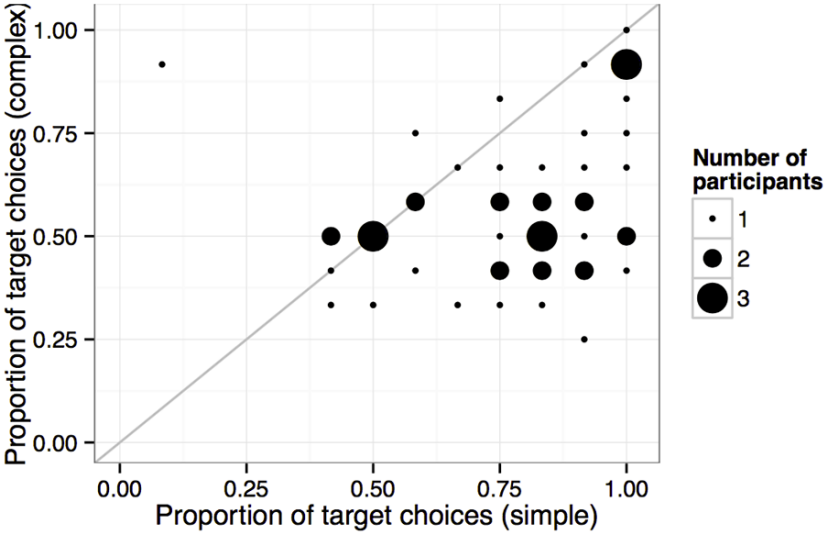
\includegraphics[width=1\linewidth]{images/l1_l2_stats.png}
  \caption{Proportion of target choices in simple and complex conditions by participant. }
  \label{fig:prob_stats}
\end{subfigure}
\caption{Plots from \cite{Franke_2016}.}
\label{fig:stats}
\end{figure}

So as one can see the $L_2$ can correctly identify the target considering the highest probability. Hence, the main point to take from here is that $L_1$ listener can solve the simple task, but cannot solve the complex one, while the $L_2$ listener is able to solve both. 

Further expending on this, the previous research shows, that the modeled listeners align with the empirical data. In particular, see \autoref{fig:stats} taken from \cite{Franke_2016}. \autoref{fig:trial_stats} shows that indeed the difficulty gets harder going from unambiguous to simple and further to complex trials. On the other hand, \autoref{fig:prob_stats} shows that there are roughly 3 clusters present depending on whether one can solve only simple, both or neither of trials. This strongly supports the alignment with $L_0,L_1$ and $L_2$ listeners. However, very important to note that we are only talking about the alignment of RSA model's accuracy with the empirical data, while the concrete strategies are not taken into account.

Now we will proceed further, and make a hypothesis about how people could be solving these problems. A key difference between simple and complex trials is the fact that solving complex trials requires one to consider the distractor as well due to the matching feature with the target, while in the simple one, the distractor can be ignored completely. This can be demonstrated by the following matrix transformations. If one does not take into account the distractor the $M_s,M_c$ will instead look as in \autoref{eq:8} and \autoref{eq:9} correspondingly. 

\begin{equation} \label{eq:8}
M_s' = \!\!\!\!
\raisebox{2.3ex}{$
\begin{array}{c@{\;}c}
    & {
    \begin{array}{*{4}{C{20pt}}} 
        \inlinegraphics{images/shapes_and_colors/blue_square.png} & \inlinegraphics{images/shapes_and_colors/blue_circle.png}  
      \end{array}} \\[5pt]
    \begin{array}{c} 
        \inlinegraphics{images/shapes_and_colors/blue.png} \\ 
        \inlinegraphics{images/shapes_and_colors/circle.png} \\ 
        \inlinegraphics{images/shapes_and_colors/green.png} \\
        \inlinegraphics{images/shapes_and_colors/triangle.png}
    \end{array} 
    & 
    \left[
    \begin{array}{*{2}{C{20pt}}}
        1 & 1  \\
        0 & 1  \\
        0 & 0  \\
        0 & 0  \\
    \end{array} \right]
\end{array}$
}
\end{equation}

\begin{equation} \label{eq:9}
M_c' = \!\!\!\!
\raisebox{2.3ex}{$
\begin{array}{c@{\;}c}
    & {
    \begin{array}{*{4}{C{20pt}}} 
        \inlinegraphics{images/shapes_and_colors/blue_square.png} & \inlinegraphics{images/shapes_and_colors/blue_circle.png}
      \end{array}} \\[5pt]
    \begin{array}{c} 
        \inlinegraphics{images/shapes_and_colors/blue.png} \\ 
        \inlinegraphics{images/shapes_and_colors/circle.png} \\ 
        \inlinegraphics{images/shapes_and_colors/square.png} \\
        \inlinegraphics{images/shapes_and_colors/triangle.png}
    \end{array} 
    & 
    \left[
    \begin{array}{*{3}{C{20pt}}}
        1 & 1 \\
        0 & 1 \\
        1 & 0 \\
        0 & 0 \\
    \end{array} \right]
\end{array}$
}
\end{equation}

Applying $L_1$ transformation to the $M_s'$ we get \autoref{eq:10} which accomplishes the same as in \autoref{eq:4}.

\begin{equation} \label{eq:10}
L_1(M_s') = \!\!\!\!
\raisebox{2.3ex}{$
\begin{array}{c@{\;}c}
    & {
    \begin{array}{*{4}{C{20pt}}} 
        \inlinegraphics{images/shapes_and_colors/blue_square.png} & \inlinegraphics{images/shapes_and_colors/blue_circle.png}  
      \end{array}} \\[5pt]
    \begin{array}{c} 
        \inlinegraphics{images/shapes_and_colors/blue.png} \\ 
        \inlinegraphics{images/shapes_and_colors/circle.png} \\ 
        \inlinegraphics{images/shapes_and_colors/green.png} \\
        \inlinegraphics{images/shapes_and_colors/triangle.png}
    \end{array} 
    & 
    \left[
    \begin{array}{*{2}{C{20pt}}}
        0.66 & 0.33  \\
        0 & 1  \\
        0 & 0  \\
        0 & 0  \\
    \end{array} \right]
\end{array}$
}
\end{equation}

On the other hand, neither $L_1$ nor $L_2$ can solve the matrix $M_c'$. In fact no depth of recursion is helpful in this case as $L_0(M_c')=L_1(M_c')=L_2(M_c')$ (\autoref{eq:11}).

\begin{equation} \label{eq:11}
L(M_c') = L(S(M_c')) = L(S(L(M_c'))) = \!\!\!\!
\raisebox{2.3ex}{$
\begin{array}{c@{\;}c}
    & {
    \begin{array}{*{4}{C{20pt}}} 
        \inlinegraphics{images/shapes_and_colors/blue_square.png} & \inlinegraphics{images/shapes_and_colors/blue_circle.png}
      \end{array}} \\[5pt]
    \begin{array}{c} 
        \inlinegraphics{images/shapes_and_colors/blue.png} \\ 
        \inlinegraphics{images/shapes_and_colors/circle.png} \\ 
        \inlinegraphics{images/shapes_and_colors/square.png} \\
        \inlinegraphics{images/shapes_and_colors/triangle.png}
    \end{array} 
    & 
    \left[
    \begin{array}{*{3}{C{20pt}}}
        0.5 & 0.5 \\
        0 & 1 \\
        1 & 0 \\
        0 & 0 \\
    \end{array} \right]
\end{array}$
}
\end{equation}

This leads us to a research question of whether people achieve $L_1$ accuracy by not considering the distractor and applying reasoning deeper than one of a literal speaker. Or they include the distractor in their reasoning but simply lack the depth of recursion therefore failing to solve the complex trials.




\section{How Eye Tracking is Useful}
\begin{figure}
    \centering
    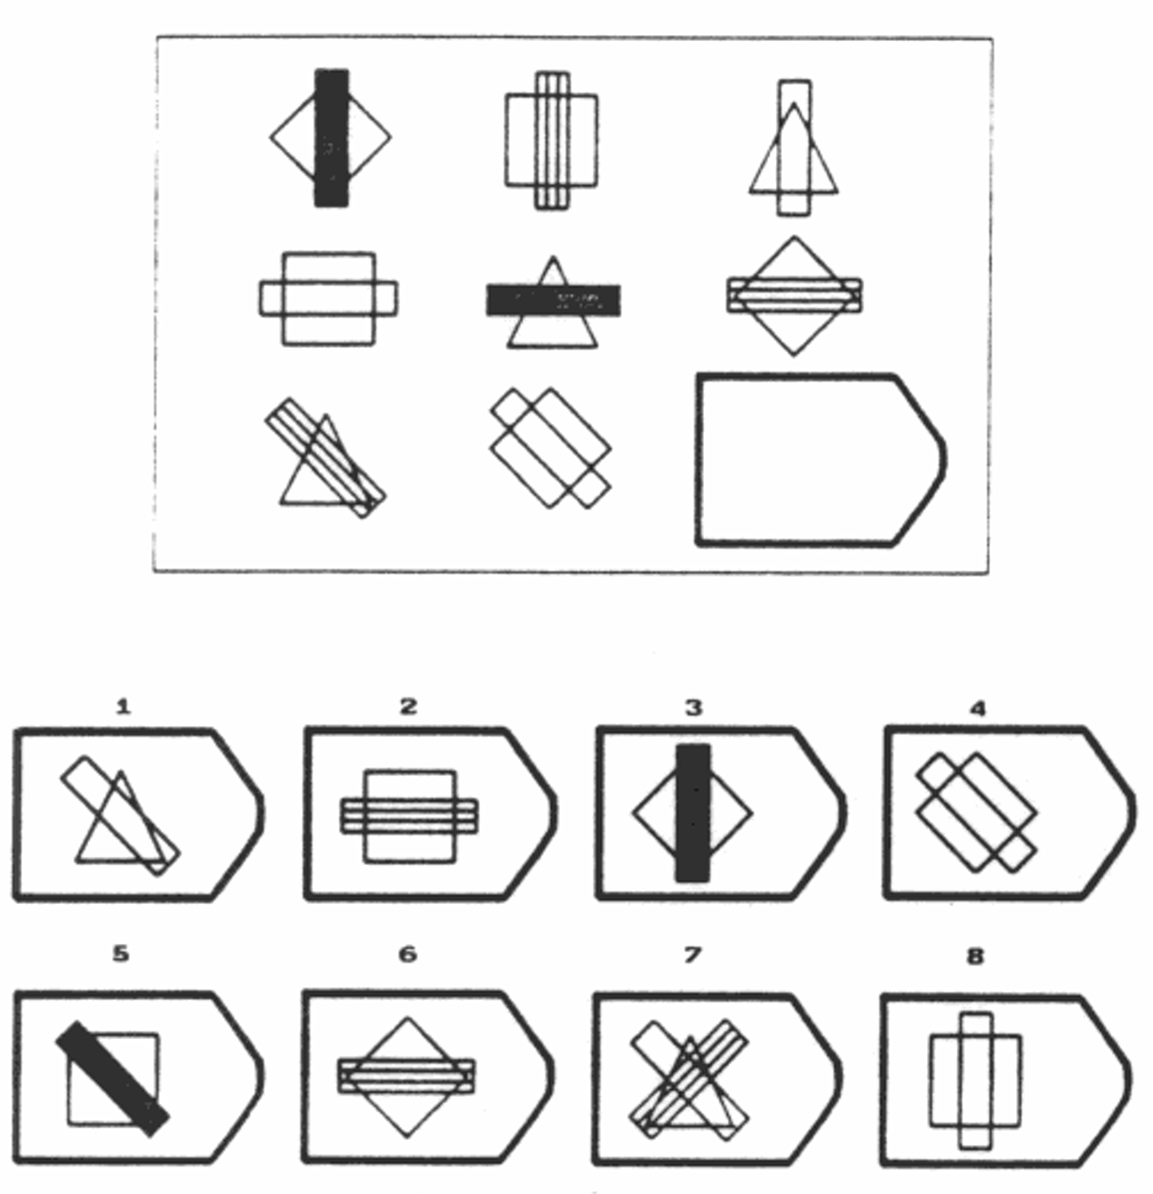
\includegraphics[width=0.5\linewidth]{images/raven_carpenter_1990.png}
    \caption{An example of Raven item. The upper part is the matrix, while the bottom is possible answers. The matrix is constructed as follows. The lines orientation is constant within rows. While the shapes and line appearances are obeying the distribution-of-three-values rule. Simply put same three values are present in each row. The correct answer is 5.}
    \label{fig:raven}
\end{figure}
We will take a look at a related field with different kind of tasks, this strategy has shown to be particularly informative and insightful there. 
The Raven Progressive Matrices, commonly referred to as the Raven Tests, are a set of nonverbal intelligence tests designed to measure abstract reasoning and problem-solving abilities through pattern recognition and logical inference. Such test usually contains 8 objects arranged in a 3 by 3 grid with one object missing, as well as the set of possible answers displayed below the matrix. Each matrix either has a particular rule it is constructed by or a mix of them. An example is presented in \autoref{fig:raven}. 

Researches suggest that there are two main strategies for solving the Raven Tests constructive matching and response elimination \citep{Bethel-Fox_1984} and later followed by \cite{Vigneau_2006}. The former is described as successively finding rules by which the matrix is constructed, until the answer is fully derived. And the later means that rather than going through the matrix, one goes over the possible answers and eliminates them one by one, ending up with the correct one in the end. The less efficient of these, response elimination, seemed to be used more by lower ability subjects on more difficult items. 

The two strategies can be identified by the patterns of one's attention, hence, eye gaze. The constructive matching being focused on the matrix and systematically going through rows and columns of it. \cite{Carpenter_1990} expand on the eye tracking experiments in this research question by recording eye gaze as well as the verbal comments during the process of solving the tasks. A very detailed sequence of actions is acquired therefore giving an insight into how one uses the constructive matching strategy to solve Raven Progressive Matrices. On the other hand, the response elimination involves a lot of toggling between the possible answers and the matrix. In order to deepen the understanding in this problem \cite{Vigneau_2006} develop a set of features to encode ones attention. Such features include for example Time on Matrix, Time on Alternatives (possible answers) or Number of Toggles between the possible answers and the matrix. The authors proceed to report the correlation between the features and the percent of ones correct answers. Indeed, the results show statistically significant negative correlation of Time on Alternatives and Number of Toggles with overall score. These findings further supports theory about the difference in effectiveness in the two strategies. 


One can see based on these studies why and how the eye tracking is useful in the reference games. In our case as discussed in the end of \autoref{sec:rsa} there are multiple ways people could reach $L_1$ accuracy. Therefore suggesting that the two potential strategies would be distinguished by the use of distractor. At the same time, there are still $L_0$ and $L_2$ listeners present in the experiment which makes the distinction more difficult. On the other hand, as there is no previous work on eye tracking reference games, the study is also highly exploratory.

\section{Out of Lab Eye Tracking} \label{sec:eyetr}
\begin{figure}
    \centering
    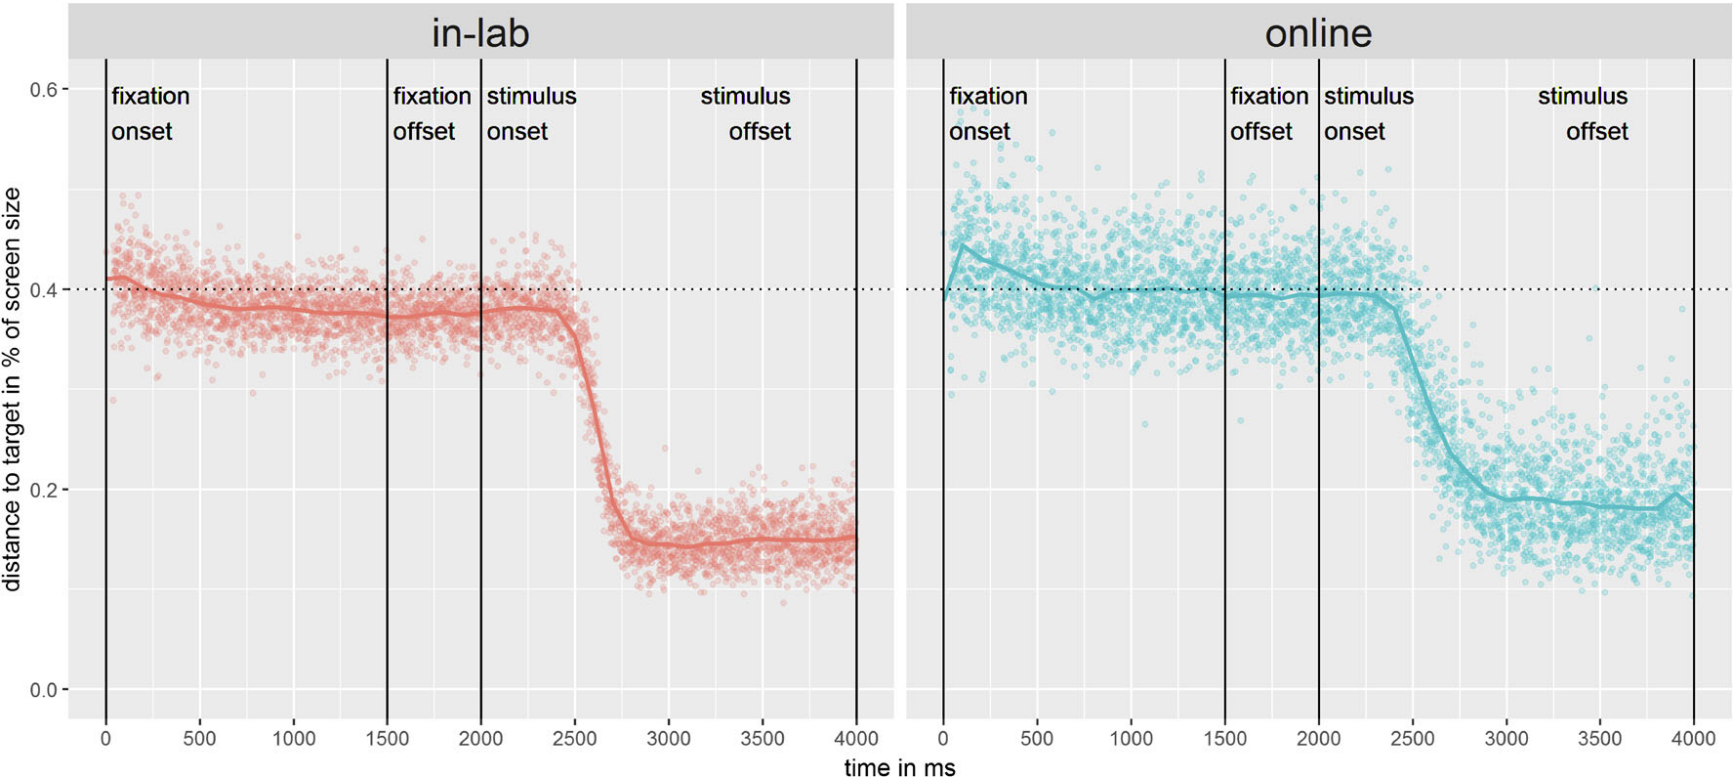
\includegraphics[width=1\linewidth]{images/tracker_comparison.png}
    \caption{Figure from \cite{Semmelmann_2018}. Fixation task results. Each dot denotes a single recorded data point in distance to a target in percentage of screen size over time.}
    \label{fig:eyetr_comparison}
\end{figure}
Up until now most of the eye tracking studies have been using the laboratory equipment in order to conduct the experiments. This is very important as a reliable and precise method is needed for such experiments. On the other hand, this approach requires people to be physically present in the laboratory, which makes the experiment far more difficult to conduct in comparison to participants answering a series of questions on their laptops. Hence, a different approach was chosen. This experiment will incorporate participants' webcams to get collect the eye tracking part of the data. In particular a library called WebGazer is used \cite{webgazer}. Details about the implementation will be discussed in the following sections. 

Although, on the first glance, the effectiveness of such approach can be debatable, there is work in favor of the method. Starting from the article \cite{Semmelmann_2018} where they take a look into online webcam-based eye tracking comparing it to a respective in-lab experiment. Along with a more fresh research article which also makes this comparison \citep{Wisiecka_2022}. Both of them conclude that while WebGazer is still inferior to the lab equipment in terms of precision, the measurements are reasonably accurate. In particular, taking a look at the results of \cite{Semmelmann_2018} shown in \autoref{fig:eyetr_comparison}. This figure depicts a particular fixation on the target which was shown after 2000 ms. It takes some time for one to react and for the software to capture the eye movement. Then we observe the saccade in both settings, on average the saccade took 450 ms (750 ms in the online case). The accuracy was 171 px (207 px online), which translates to about 3.94° visual angle in the in-lab setting. In addition, it is visible that the online setting has higher variance.

Taking into account the fact that each problem statement by itself consists of multiple objects located on one page, it is not hard to setup them far apart to mitigate the decline in precision. The shorter saccade length is not of the essence in our case.

\chapter{Concept}
 
Previous work on individual differences \cite{Franke_2016} has focused on differences in underlying pragmatic reasoning tendencies. However participants with the same underlying pragmatic tendencies may underperform based on the information in the problem that they pay attention to. Take for example the hypothesis we saw in \autoref{sec:rsa}, there not paying attention to the distractor would mean that the problem simply becomes unsolvable. Therefore, cognitive abilities such as attention and working memory are most likely not the only features contributing to the performance of participants in these tasks.

This thesis aims to shed light on the realm of where the attention is spent during the pragmatic reasoning problem-solving task. And the eye tracking data will be used to investigate this. 

\section{Research Questions}
\label{sec:research_questions}

\subsection{Estimating the Posterior}
\label{sec:posterior}
At first, we are interested in predicting the posterior, that is the probability of a participant to solve a problem give the eye gaze features as well as the general information about the trial.

\subsubsection{Research Hypothesis 1}
\label{sec:h1}
As we discussed in \autoref{sec:rsa}, the distractor in the hypothesis is a crucial part of the problem. Therefore, it is important to understand how participants interact with the distractor. The first research hypothesis is H1: Proportional time on distractor is positively associated with accuracy on Complex trials.

\subsubsection{Research Hypothesis 2}
\label{sec:h2}
The second research question is about the messages that are available to the participants. The second research hypothesis is H2: Proportional time on available messages is positively associated with accuracy on Simple trials. This hypothesis is mainly based on the idea that while the unambiguous trials can be solved without considering the available messages, the simple ones require one to consider the available messages. In addition, the Complex trials can be solved without looking at the available messages.

\subsection{Estimating the Likelihood}
\label{sec:likelihood}

Because of the same patterns of information, we expect that skilled participants should in general have a different attention profile in Simple trials than in Complex trials. Therefore, we would like to do a slightly alternative analysis, estimating the likelihood directly instead of trying to estimate the posterior. In order to realize this, we will only take the correctly solved trials into account and predict the probability of a each fixation to be on the area of interest.

\subsubsection{Research Hypothesis 3}
\label{sec:h3}
The third research hypothesis is H3: on correctly solved trials, Complex trial condition is positively associated with the probability of fixation being on the distractor. 

\subsubsection{Research Hypothesis 4}
\label{sec:h4}
The fourth research hypothesis is H4: on correctly solved trials, Simple trial condition is positively associated with the probability of fixation being on the available messages.



\chapter{Implementation}

\section{Data Collection}
\label{sec:data}

\subsection{Reference Games}
\label{sec:data:ref_games}

\subsection{Eye Tracking}
\label{sec:data:eyetr}

\section{Analysis}
\label{sec:analysis}

\subsection{Pairwise Correlations}
\label{sec:analysis:corr}

\subsection{Mixed Effects Logistic Regressions}
\label{sec:analysis:mixed_effects}

\subsection{Exploratory Analysis}
\label{sec:analysis:exploratory}

\subsubsection{Clustering}
\label{sec:analysis:exploratory:clustering}

\subsubsection{CNNs}
\label{sec:analysis:exploratory:cnn}

\chapter{User Study}
\chapter{Conclusion and General Discussion}
\label{chap:conclusion}

\section{Conclusion}
\label{sec:conclusion}

In this thesis, we approached the research question from multiple analytical angles to better understand how visual attention relates to reasoning in reference games. First, we conducted a pairwise correlation analysis between eye-tracking features and two key trial-level outcomes: accuracy and response time. Next, we built a logistic regression model to predict whether a given trial would be solved correctly, based on the participant's gaze behavior. To further investigate the role of attention, we implemented two additional logistic regression models that focused on specific fixation patterns: one predicted whether a gaze point would land on the Distractor, and the other did the same for the bank of available messages. Finally, we analyzed participants' self-reported strategies and labeled them according to the Rational Speech Act (RSA) framework ($L_0$, $L_1$, $L_2$). This allowed us to compare how different reasoning strategies manifest in distinct attentional profiles.

Although participants seem to grasp the problem in a similar way, their answers still differ quite a lot. We saw this from the fact that the Distractor did not turn out to be associated with accuracy, even though it is a very important piece of information for the Complex trials. Thus, participants fail the trials not because they miss an important piece of information as we hypothesized in \autoref{sec:rsa}, where we showed that not looking at the Distractor would make the Complex condition unsolvable. The problem appears to lie in how participants interpret or apply the information they attend to, rather than in what information they access.

The consistent association between accuracy and proportional time spent on the bank of available messages suggests that this behavior may reflect more than simple visual scanning. It is plausible that participants engage in matching messages to objects, or in other forms of referential reasoning. In the context of reference games, such (possibly recursive) reasoning processes are essential. Thus, increased attention to the available messages may serve as an indicator of deeper or more robust reasoning, ultimately leading to higher accuracy.

While we could not directly infer participants' reasoning strategies, we were able to identify eye-tracking features associated with trial accuracy. Further research might include more sophisticated analysis to identify the actual strategies of the participants. The main finding suggests that the bank of available messages is an important area of interest when predicting whether a person is going to solve the trial correctly. A possible future work might include detecting which messages the participants are looking at and how they are using them. This reflects a design limitation: anticipating potential quality issues with WebGazer, we placed the available messages close together -- thus sacrificing the ability to detect which message the participants are looking at. However, this is a very interesting question and could be a good future work.

Ongoing research on modeling participant behavior in reference games using ACT-R \citep{Duff_2025} may provide deeper insights into the cognitive strategies underlying their responses.

This thesis contributes to a wider ongoing research on reference games. Overall, this work demonstrates that even with limited-resolution eye-tracking data, meaningful patterns can be extracted that shed light on participants' reasoning processes in reference games. This thesis provides a strong foundation for future work that would include eye-tracking data in reference games or another type of experiment with a similar setup. 


\section{General Discussion}
\label{sec:general-discussion}

\subsection{Scanpaths}
\label{sec:general-discussion:scanpaths}
In this study, did not account for  the order of the gaze points. However, the scanpath by itself includes this information. We were unable to come up with a good strategy how one could encode the scanpath in a way that would be useful and feasible for the analysis. The scanpaths are not fixed length, posing a problem that every entry would be of a different length which would make it impossible to use them in a model. One idea could be to use RNNs to analyze the scanpaths, however, this would require a lot of data and a lot of tuning. We did a few attempts in training CNNs on the generated plots of the scanpaths, however, the results were not promising and due to low interpretability of the model and time constraints we decided to focus on the more traditional features.

\subsection{Peripheral Vision}
\label{sec:general-discussion:attention-and-eye-tracking}
It is possible that the participants used their peripheral vision to look at the objects. If one specifically tries to solve the trial without moving the eyes, one could still do it. This definitely poses a problem for the eye tracking data, as it would be impossible to detect this kind of behavior. We do not have any evidence that this is the case, but it is a possibility. People would not specifically try to solve the trials without the eye movements, however, it is quite probable that they capture some features such as color of the Distractor in case that the sent message is a shape during the trial. This is somewhat supported by the likelihood model predicting whether a gaze point would end up on the Distractor or not \autoref{sec:distractor_model}. \texttt{MsgType} had a very low but significant coefficient indicating exactly this behavior. Although this is not a strong evidence for the peripheral vision, the potential problem should be taken into account.


\subsection{Toggling}
\label{sec:general-discussion:toggling}
We only implemented features that describe proportional time spent on the area of interest. However, as we described in the \autoref{sec:conclusion}, an increase in proportional time on available messages might indicate a deeper reasoning process. One could also think about defining a feature to describe the toggling between the available messages and other areas of interest. Similarly to how it was done in \cite{Vigneau_2006}. The toggling might be an important predictor for accuracy if one makes repeated matches of the messages and the objects. 

\subsection{Proportional Eye Tracking Features}
\label{sec:general-discussion:proportional-eye-tracking-features}
We suspect that the proportional eye tracking features might be influence by the very last look at one of the objects. Therefore, making them good predictors of accuracy, as we saw in \autoref{sec:accuracy_model} or \autoref{sec:pairwise_corr}. The Competitor and Distractor turned out to be decisive for the accuracy of the predictions. This indicates that people look more at the object they would choose. As for the future work, one should consider trimming the last saccade before the decision, this should make the proportional features more reliable. On the other hand, if this does not solve the issue, this would indicate that people tend to make a decision not in the end of the trial. This would be also be an interesting finding.

The way we assigned the fixations to the stimuli is not optimal as we clearly disregarded the timings of the gaze predictions as well as added some of the gaze points that are from saccades rather than from fixations. Both of the problems could have been solved with a fixation detection algorithm. A more advanced fixation detection algorithm could be implemented in the future to improve the preprocessing part of the data analysis. Currently as was discussed in \autoref{sec:analysis:eyetr} the fixation detection algorithm falls short in the case of low sampling rates that WebGazer demonstrates. The algorithm is unable to detect some fixations in the data, which can lead to a loss of information.

\subsection{Eye Tracking}
\label{sec:general-discussion:eye-tracking}
The eye tracking data collected by WebGazer was definitely worse than one could collect in the lab. However, clearly this thesis is an example that it is possible to conduct an eye tracking experiment with WebGazer. The data is not perfect, but it is good enough to be able to draw some conclusions from it. However, the library is far from perfect and definitely needs a lot of adjustments to the specific setups one could be interested in. Designing the experiment took far more time than the actual analysis of the data. Each participant has a different setup. And, although, the calibration of the eye tracker must be conducted quite strictly, it is also important to make sure that the calibration is doable for the participants. We have achieved some balance between the two, but it is still not perfect. 

On the other hand, WebGazer has a few clear advantages. First of all, the fact that it is possible to collect data from a large number of participants. This is something that is not possible in the lab, especially for an eye tracking study as it would require individual treatment of each participant, as oppose to each participant working in parallel in the online experiment. Secondly, WebGazer is free and open source, which makes it available for everyone. This is a clear advantage over the lab eye trackers that are expensive and not available for everyone. 

\appendix
\clearpage
\addcontentsline{toc}{chapter}{Appendices}
\chapter*{Appendices}

\chapter{Appendix A: Additional Details}
\label{appendix:a}
% Add content for Appendix A here
\section{Pairwise Correlations}
\label{sec:pairwise_corr_unambiguous}

\begin{table}[h!]
\centering
\begin{tabular}{|l|c|c|c|c|}
\hline
\textbf{Feature} & \textbf{Mean} & \textbf{SD} & \textbf{Accuracy} & \textbf{Mean Answer Time} \\ \hline
PropTimeOnSentMsg & 0.46 & 0.11 & 0.12 & -0.38 *** \\ \hline
PropTimeOnAvailableMsgs & 0.03 & 0.03 & -0.1 & 0.43 *** \\ \hline
PropTimeOnTrgt & 0.24 & 0.08 & -0.04 & -0.0 \\ \hline
PropTimeOnDist & 0.12 & 0.06 & -0.13 & 0.25 * \\ \hline
PropTimeOnComp & 0.12 & 0.06 & -0.01 & 0.2 * \\ \hline
PropTimeOnNonAOI & 0.02 & 0.02 & 0.11 & 0.15 \\ \hline
MeanAnswerTime & 3005.96 & 2179.31 & -0.1 & --- \\ \hline
AnswerAccuracy & 0.99 & 0.05 & --- & --- \\ \hline
\end{tabular}
\caption{Unambiguous condition. Correlation table showing the relationships between features, accuracy, and mean answer time. Significance levels: * $p < 0.05$, ** $p < 0.01$, *** $p < 0.001$.}
\label{tab:feature_summary}
\end{table}

The table above shows the pairwise correlation between the features, accuracy, and mean answer time in the Unambiguous trials. There were no significant correlations between the features and accuracy. The only significant correlations were in the Mean Answer Time column, the results are not surprising as the Unambiguous trials are not difficult to solve, and most of the participants adopted a similar strategy where they would just match the sent message with the only object that has the same feature. This strategy involves only looking at sent message and the Target, making any deviations indicate that the participant is not following the strategy and they will take longer on the trial. It is worth to mention, that while the strategy is very efficient, a deviation from it does not make one answer incorrectly as can be seen from the results.


\chapter{Appendix B: Supplementary Material}
\label{appendix:b}


\section{Trials}
\begin{table}[H]
\centering
\resizebox{\textwidth}{!}{%
\begin{tabular}{|c|c|c|c|c|c|c|c|c|c|}
\hline
ID & Condition & Sent Msg & Trgt & Comp & Dist & Msg1 & Msg2 & Msg3 & Msg4 \\ \hline
1  & simple & ci & ci\_bl & ci\_gr & tr\_re & ci & tr & re & gr \\ \hline
2  & simple & re & tr\_re & sq\_re & ci\_bl & re & bl & ci & sq \\ \hline
3  & simple & ci & ci\_bl & ci\_gr & sq\_re & ci & sq & re & gr \\ \hline
4  & simple & re & sq\_re & tr\_re & ci\_gr & re & gr & ci & tr \\ \hline
5  & simple & sq & sq\_bl & sq\_gr & tr\_re & sq & tr & re & gr \\ \hline
6  & simple & gr & tr\_gr & ci\_gr & sq\_bl & gr & bl & sq & ci \\ \hline
7  & simple & sq & sq\_bl & sq\_gr & ci\_re & sq & ci & re & gr \\ \hline
8  & simple & gr & ci\_gr & tr\_gr & sq\_re & gr & re & sq & tr \\ \hline
9  & simple & tr & tr\_bl & tr\_gr & sq\_re & tr & sq & re & gr \\ \hline
10 & simple & bl & sq\_bl & ci\_bl & tr\_gr & bl & gr & tr & ci \\ \hline
11 & simple & tr & tr\_bl & tr\_gr & ci\_re & tr & ci & re & gr \\ \hline
12 & simple & bl & ci\_bl & sq\_bl & tr\_re & bl & re & tr & sq \\ \hline
13 & complex & ci & ci\_gr & ci\_re & sq\_gr & ci & tr & re & gr \\ \hline
14 & complex & re & sq\_re & ci\_re & sq\_gr & re & bl & ci & sq \\ \hline
15 & complex & ci & ci\_gr & ci\_re & tr\_gr & ci & sq & re & gr \\ \hline
16 & complex & re & tr\_re & ci\_re & tr\_bl & re & gr & ci & tr \\ \hline
17 & complex & sq & sq\_gr & sq\_re & ci\_gr & sq & tr & re & gr \\ \hline
18 & complex & gr & ci\_gr & sq\_gr & ci\_re & gr & bl & sq & ci \\ \hline
19 & complex & sq & sq\_gr & sq\_re & tr\_gr & sq & ci & re & gr \\ \hline
20 & complex & gr & tr\_gr & sq\_gr & tr\_bl & gr & re & sq & tr \\ \hline
21 & complex & tr & tr\_gr & tr\_re & ci\_gr & tr & sq & re & gr \\ \hline
22 & complex & bl & ci\_bl & tr\_bl & ci\_re & bl & gr & tr & ci \\ \hline
23 & complex & tr & tr\_gr & tr\_re & sq\_gr & tr & ci & re & gr \\ \hline
24 & complex & bl & sq\_bl & tr\_bl & sq\_gr & bl & re & tr & sq \\ \hline
25 & unambiguous & ci & ci\_re & sq\_re & sq\_bl & ci & sq & re & gr \\ \hline
26 & unambiguous & re & ci\_re & ci\_gr & tr\_gr & re & gr & ci & sq \\ \hline
27 & unambiguous & ci & ci\_re & tr\_re & tr\_bl & ci & tr & re & gr \\ \hline
28 & unambiguous & re & ci\_re & ci\_bl & sq\_bl & re & bl & ci & tr \\ \hline
29 & unambiguous & sq & sq\_re & ci\_re & ci\_bl & sq & ci & re & gr \\ \hline
30 & unambiguous & gr & sq\_gr & sq\_re & tr\_re & gr & re & sq & ci \\ \hline
31 & unambiguous & sq & sq\_re & tr\_re & tr\_bl & sq & tr & re & gr \\ \hline
32 & unambiguous & gr & sq\_gr & sq\_bl & ci\_bl & gr & bl & sq & tr \\ \hline
33 & unambiguous & tr & tr\_re & ci\_re & ci\_bl & tr & ci & re & gr \\ \hline
34 & unambiguous & bl & tr\_bl & tr\_re & sq\_re & bl & re & tr & ci \\ \hline
35 & unambiguous & tr & tr\_re & sq\_re & sq\_bl & tr & sq & re & gr \\ \hline
36 & unambiguous & bl & tr\_bl & tr\_gr & ci\_gr & bl & gr & tr & sq \\ \hline
37 & strtgy\_simple & ci & ci\_bl & ci\_gr & tr\_re & ci & tr & re & gr \\ \hline
38 & strtgy\_complex & bl & sq\_bl & tr\_bl & sq\_gr & bl & re & tr & sq \\ \hline
\end{tabular}%
}
\caption{Table of all trials used in the experiment. }
\label{tab:trials}
\end{table}


%  !!!!!!!!!!!!!!!!!!!!!! !!!!!!!!!!!!!!!!!!!!!! !!!!!!!!!!!!!!!!!!!!!! !!!!!!!!!!!!!!!!!!!!!! !!!!!!!!!!!!!!!!!!!!!! !!!!!!!!!!!!!!!!!!!!!!
% Please ensure that the bibliography is consistent! That means (amongst other things): 
%- Conferences should always be named the same. I.e., if you cite papers that appeared at the same conference series, check that the names are identical in these two entries (besides the year)
%- If one of your titles is capitalized, ensure that all of them are capitalized. 
%- The same pieces of information should be denoted for every entry. I.e., if you have provided the publisher in one entry, you should show the publisher for every entry. You have used the DOI at least once? Then use it for every entry.
%- Please check the consistency before a hand-in occurs. 

%NOTE: You are allowed to change the bibliographystyle. 


	\cleardoublepage
\begingroup
	\phantomsection
  \pagestyle{plain}
  \bibliographystyle{apacite}
   \phantomsection
	\addcontentsline{toc}{chapter}{Bibliography}
	\interlinepenalty=10000 %prevents bibtex that are one two pages.
	\bibliography{references}\emph{}	
	\vfill
  \clearpage
\endgroup 
\end{document}
